%% -*- mode: LaTeX -*-
%%

%%%%%%%%%%%%%%%%%%%%%%%%%%%%%%%%%%%%%%%%%%%%%%%%%%%%%%%%%%%%%%%%%%%%%%%%%%%%%%%

\section{Measurement Methodology}
\label{sec:methodology}

\begin{figure}
  \centering
  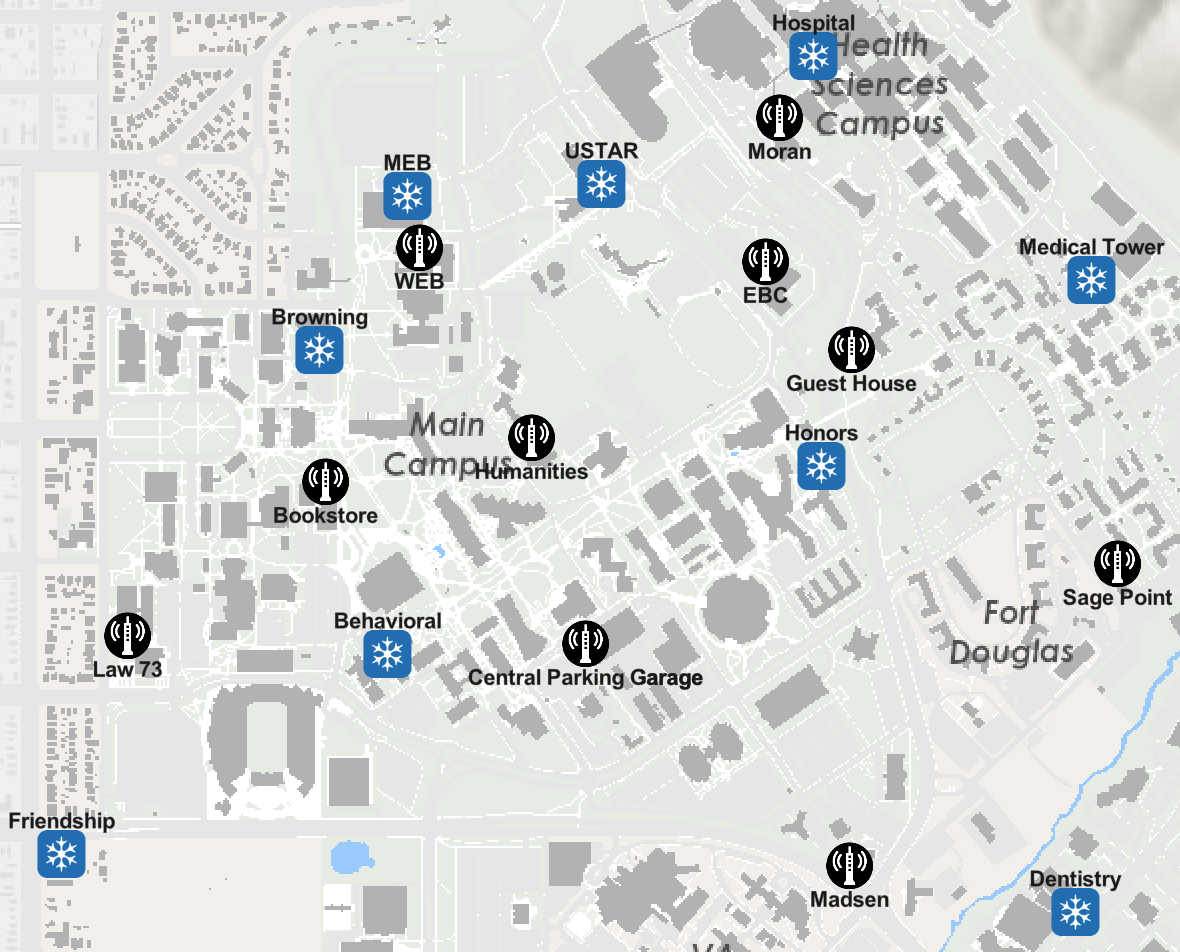
\includegraphics[width=0.9\columnwidth]{currPowder}
  \caption{POWDER map. Snowflakes represent base stations. Black circles represent fixed endpoint nodes ~\cite{Breen+:wintech20}.}
  \label{fig:powdernodes}
\end{figure}

Our measurement is conducted on the POWDER platform (Figure~\ref{fig:powdermap}). Most of our experiments focused on a campus
environment with a variety of terrain. Part of the area includes a typical spread out university campus, while other parts include a more densely 
populated urban-like environment. POWDER offers 9 general purpose rooftop base stations (Figure~\ref{fig:basestat}) that include networked software-defined-radios (X310s), a radio frequency front-end (time division duplex and frequency division duplex), and signal 
amplification. Furthermore, POWDER offers 10 fixed endpoints (Figure~\ref{fig:endpoints}). Similar to the general purpose rooftop base 
stations, the components include software-defined-radios, radio frequency front-end and antenna elements. Figure~\ref{fig:powdernodes} 
provides an overview of the current nodes available to us on the POWDER platform.

\begin{figure}
  \centering
  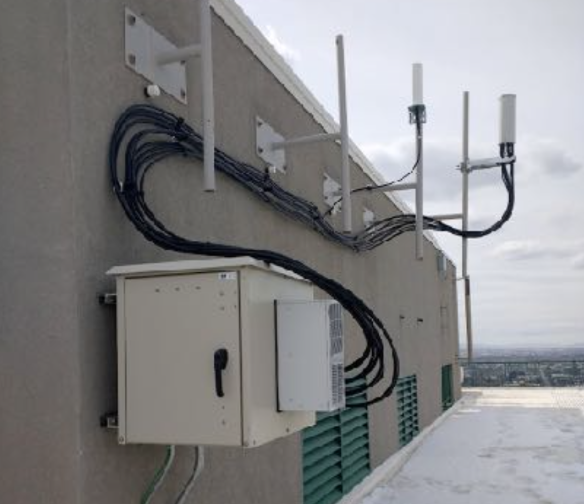
\includegraphics[width=0.9\columnwidth]{basestation}
  \caption{General purpose base station~\cite{Breen+:wintech20}.}
  \label{fig:basestat}
\end{figure}

\subsection*{Measurement Tool: Shout}

Shout~\cite{shout} is a measurements framework developed by the POWDER team. Using Shout you are able to collect radio frequency
measurements for the nodes within the testbed. The framework was developed on python and offers a rich set of measurement collections.
Shout follows a client server architecture in which we have an orchestrator node running at all times. On each client (radio node) we 
connect to the orchestrator via IP address. The orchestrator prints out commands telling us what nodes have connected. Once all chosen 
nodes have connect we can then begin the measurement process. 

For our purposes we used Shout to collect radio frequency propagation among the nodes on the platform. Shout uses JSON files as 
command files to tell the orchestrator how it should direct the other nodes. We used a configuration file which directed the framework 
to treat each node as a receiver and transmitter in a round-robin fashion. Figure~\ref{fig:allmeaspaths} shows the JSON file used to 
produce our results. Notice, that the JSON file used follows this approach:
\begin{align}
PL_M = CF + \frac{1}{2}SR
\end{align}
Where $CF$ is the center frequency (tuned frequency) and $SR$ is the sample rate. $PL_M$ describes the upper bound for collection, with 
a frequency step size dictated by the JSON file. In other words for the given $CF$ we collect measurements up to $PL_M$ with a given 
frequency step. Shout then averages these results to produce an average received power for the given frequency between two nodes. This is the 
approach we follow when calculating radio frequency propagation using the Shout framework.

\begin{figure}
  \centering
  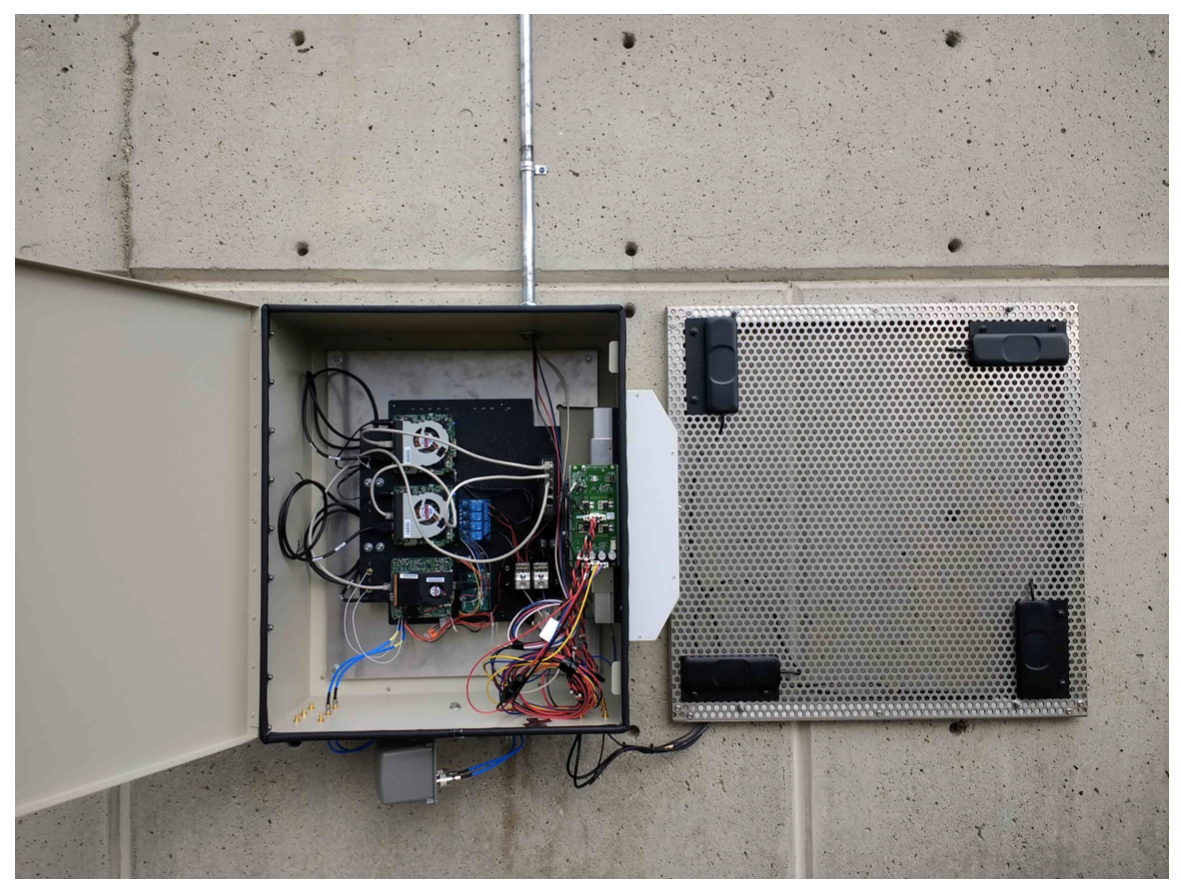
\includegraphics[width=0.9\columnwidth]{fixedEndpoint}
  \caption{Fixed endpoint~\cite{Breen+:wintech20}.}
  \label{fig:endpoints}
\end{figure}

\subsection*{Measurement Tool: SPLAT! }
SPLAT!~\cite{splat} will be our modeling tool to compare with Shout's results. SPLAT! can be used to produce terrain analysis maps of the 
designated area, but for our purposes we will use SPLAT! as a point-to-point analysis model to calculate radio frequency propagation. For radio
frequency propagation, SPLAT! requires two primary files: QTH, and LRP. QTH files are site location files that contain the site's name,
the site's latitude, the site's longitude and the site's antenna height above ground level. LRP files are the irregular terrain model parameter
files that are used to determine radio frequency path loss, field strength, or received signal power level. Figure~\ref{fig:splatFiles} shows an
example of the QTH and LRP files used on SPLAT!. Each node used on the POWDER platform was created QTH and LRP files. 

\begin{figure}
  \centering
  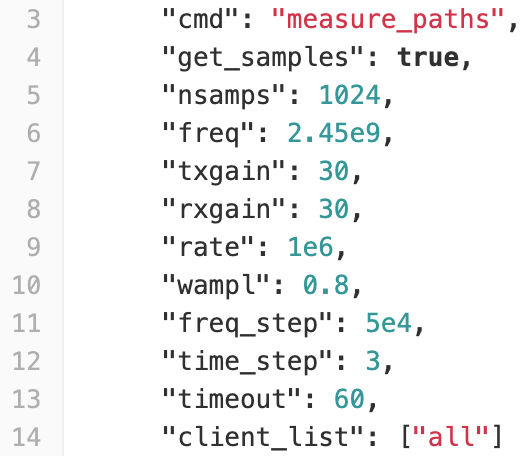
\includegraphics[width=0.9\columnwidth]{jsonFile}
  \caption{Example JSON file that tells the orchestrator how to treat the nodes. Line 3 dictates the measurement study. While line 6 and
  14 states the center frequency and which nodes to use respectively.}
  \label{fig:allmeaspaths}
\end{figure}

To produce and compare accurate results between Shout and SPLAT!, we followed the same approach as in formula (5). Using the 
proper QTH and LRP files for each node we were able to create a python script that easily mediates the process of collecting the data
for a given frequency. SPLAT! is a command-line driven application that reads in the data from the QTH and LRP files and produces a 
results file that can be parsed for the necessary data. 

\subsection*{Measurements}
Following the above methodology we perform extensive measurements on the POWDER platform using Shout and SPLAT! via
multiple frequencies and nodes. For this project we conducted 4 measurement runs with each run being done 3 times. These 
4 measurement runs span over 3 different frequency bands. To summaries: 
\begin{itemize}
  \item Run 1 took place in early October. The measurement conducted used the 3561 MHz frequency, and used the: Behavioral Science, Browning, Friendship Manor, Sagepoint, MEB, and South Medical Tower nodes. This run was conducted at mid-day. 
  
  \item Run 2 took place in early November. The measurement conducted used the 2620 MHz frequency, and used the: Behavioral Science, Browning, Friendship Manor, Honors, Sagepoint, Ustar as transmitters nodes. And used Bookstore, EBC, Garage, Guesthouse, Humanities, Law73, Madsen, Moran, and WEB as receiver fixed endpoint nodes. This run does not follow the typical round-robin approach among all the nodes where each one acts as a receiver and transmitter because only the transmitter nodes listed where able to transmit at the listed frequency. We still followed the approach discussed in equation (5).  This run was conducted early morning. 

%This run does not follow the typical measurement approach discussed earlier in this section, as the frequency used could only be transmitted by some of the nodes. 
% Fix this problem first
  
   \item Run 3 took place in late November. The measurement conducted used the 3550 MHz frequency, and used the: Behavioral Science, Browning, Honors, Sagepoint, South Medical Tower, Ustar, and Friendship Manor nodes. This run was conduct early morning. 
      
  \item Run 4 took place in late November. The measurement conducted used the 3690 MHz frequency, and used the: Behavioral Science, Browning, Honors, Sagepoint, South Medical Tower, Ustar, and Friendship Manor nodes. This run was conducted early morning.\end{itemize}

\begin{figure}
  \centering
  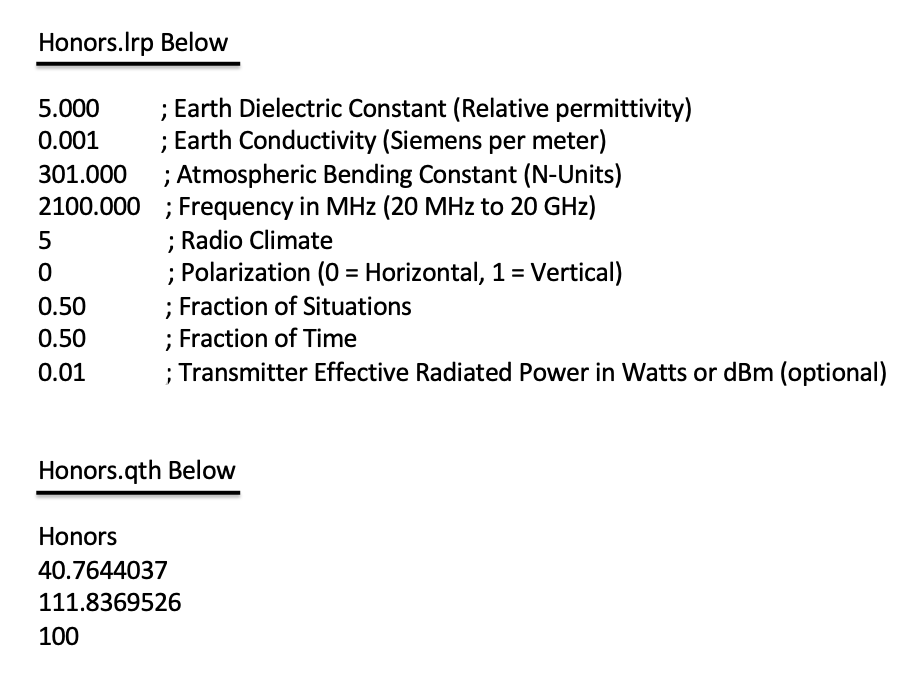
\includegraphics[width=0.9\columnwidth]{splatFiles}
  \caption{LRP and QTH SPLAT! files for Honors.}
  \label{fig:splatFiles}
\end{figure}

%%%%%%%%%%%%%%%%%%%%%%%%%%%%%%%%%%%%%%%%%%%%%%%%%%%%%%%%%%%%%%%%%%%%%%%%%%%%%%%

%% End of file.



